\newpage

\section{Введение отношения порядка на множестве параметров аппроксимирующих моделей}
В данной работе предлагается метод введения отношения порядка на множестве параметров сложных параметрических моделей, таких как нейросеть. Рассматривается порядок, заданный при помощи ковариационной матрицы градиентов функции ошибки по параметрам модели \cite{Mandt2017}. В работе \cite{Chunyan2016} предложен итерационный метод для поиска ковариационной матрицы градиентов. Данный итерационный метод интегрируется в градиентный метод оптимизации Adam \cite{Kingma2014}.

Множество параметров упорядочивается по возрастанию дисперсии: от параметра с минимальной дисперсией до параметра с максимальной дисперсией градиента функции ошибки по соответствующему параметру модели. Предполагается, что малая дисперсия градиента указывает на то, что соответствующий параметр можно зафиксировать.

Для задания порядка на множестве параметров при помощи ковариационной матрицы вводится предположение о том, что фиксация параметров происходит в момент, когда все параметры модели находятся в некоторой окрестности локального минимума функции ошибки. Данное условие накладывается для корректного использования итерационного метода поиска ковариационной матрицы градиентов.

Заданный порядок на множестве параметров модели используется для фиксации тех параметров модели, которые оказываются предстоящими с точки зрения заданного порядка. Сначала фиксируются те параметры, которые имеют минимальную дисперсию градиента в окрестности локального минимума функции ошибки.

Для анализа свойств предложенного метода задания порядка на множестве параметров проводился вычислительный эксперимент. В качестве моделей рассматривались модели различной структурной сложности: линейные модели, нейросетевые модели. Предложенный метод задания порядка сравнивается с методом, в котором порядок задан произвольным образом.
\subsection{Задача упорядочивания параметров аппроксимирующих моделей}
Задана выборка:
\[
\label{eq:st:1}
\begin{aligned}
\mathfrak{D} = \bigr\{\bigr(\textbf{x}_i, y_i\bigr)\bigr\}_{i=1}^{m}, \quad \textbf{x}_{i} \in \mathbb{X} = \mathbb{R}^{n}, \quad y_i \in \mathbb{Y},
\end{aligned}
\]
где $n$ --- размерность признакового пространства, $m$ --- число объектов в выборке. Пространство ответов $\mathbb{Y} = \mathbb{R}$ в случае задачи регрессии и  $\mathbb{Y} = \{1,\cdots, K\}$ в случае задачи классификации, где $K$ --- число классов.

Задано семейство моделей параметрических функций с наперед заданной структурой:
\[
\label{eq:st:2}
\begin{aligned}
\mathfrak{F} &= \bigr\{f\bigr(\textbf{w}\bigr):\mathbb{X} \to \mathbb{Y} | \textbf{w} \in \mathbb{R}^{p}\bigr\}, \\ 
\mathbf{h}\bigr(\textbf{w}, \textbf{x}\bigr) &= \textbf{W}_1\bm{\sigma}\bigr(\textbf{W}_2\bm{\sigma}\bigr(\cdots\bm{\sigma}\bigr(\textbf{W}_r\textbf{x}\bigr)\cdots\bigr)\bigr),\\
f_{\text{\text{cl}}}\bigr(\textbf{w}, \textbf{x}\bigr) &= \arg \max_{j \in \bigr\{1,\cdots, K\bigr\}} \text{softmax}\bigr(\mathbf{h}\bigr(\textbf{w}, \textbf{x}\bigr)\bigr)_{j}, \\ 
f_{\text{reg}}\bigr(\textbf{w}, \textbf{x}\bigr) & = \mathbf{h}\bigr(\textbf{w}, \textbf{x}\bigr), 
\end{aligned}
\]
где $p$ --- размерность пространства параметров, $r$ --- число слоев нейросети, $\textbf{w} = \text{vec}[\textbf{W}_1, \textbf{W}_2, \cdots, \textbf{W}_r]$, а $\bm{\sigma}$ --- функция активации. В случае задачи регрессии структура модели имеет вид $f_{\text{\text{reg}}}$, а в случае классификации имеет вид $f_{\text{\text{cl}}}$.
%В качестве $\tau$ рассматривается $\tau\bigr(\textbf{x}\bigr) = \textbf{x}$ в случае задачи регрессии, в случае задачи многоклассовой классификации $\bm{\sigma}\bigr(\textbf{x}\bigr) = \text{softmax}\bigr(\textbf{x}\bigr)$.
Задана функция потерь:
\[
\label{eq:st:3}
\begin{aligned}
\mathcal{L}\bigr(\textbf{w}, \mathfrak{D}\bigr) &= \frac{1}{m}\sum_{i=1}^{m}l\bigr(\textbf{x}_{i}, y_i, \textbf{w}\bigr),\\
l_{\text{\text{reg}}}\bigr(\textbf{x}, y, \textbf{w}\bigr) &= \bigr(y - f\bigr(\textbf{w}, \textbf{x}\bigr)\bigr)^{2},\\
l_{\text{\text{cl}}}\bigr(\textbf{x}, y, \textbf{w}\bigr) &= -\sum_{j=1}^{K}\bigr([y = j]\ln\text{softmax}_j\bigr(\mathbf{h}\bigr(\textbf{w}, \textbf{x}\bigr)\bigr)\bigr),
\end{aligned}
\]
где $l_{\text{\text{reg}}}$ --- это функция ошибки на одном элементе для задачи регрессии, $l_{\text{\text{cl}}}$ --- для задачи классификации.
Оптимальный вектор параметров $\hat{\textbf{w}}$ получим минимизацией функции потерь:
\[
\label{eq:st:0:1}
\begin{aligned}
\hat{\textbf{w}} = \arg \min_{\textbf{w}\in\mathbb{R}^{p}} \mathcal{L}\bigr(\textbf{w}, \mathfrak{D}\bigr).
\end{aligned}
\]

Для поиска оптимальных параметров модели используется градиентный метод оптимизации:
\[
\label{eq:st:4}
\begin{aligned}
\textbf{w}_{t} = \textbf{w}_{t-1} + \Delta\textbf{w}\bigr(\textbf{g}_{S,t}, \textbf{w}_{t-1}, \textbf{w}_{t-2}, \cdots\bigr), \quad \textbf{g}_{S,t}=\frac{\partial \mathcal{L}\bigr(\textbf{w}_{t}, \textbf{X}_{S}, \textbf{Y}_{S}\bigr)}{\partial \textbf{w}},
\end{aligned}
\]
где $t$ --- номер итерации, $\textbf{g}_{S,t}$ --- значение градиента на подвыборке размера $S$, $\Delta\textbf{w}$ --- приращение вектора параметров.
 
 
Порядок на множестве параметров модели задается при помощи ковариационной матрицы $\textbf{C}$ градиентов функции ошибки $\mathcal{L}$ по параметрам модели $\textbf{w}$. Для вычисления ковариационной матрицы $\textbf{C}$ используется итерационная формула \cite{Chunyan2016}, которая вычисляется на каждой итерации \eqref{eq:st:4} градиентного метода оптимизации параметров:
\[
\label{eq:st:5}
\begin{aligned}
\textbf{C}_t = \bigr(1-\kappa_t\bigr)\textbf{C}_{t-1}+\kappa_t\bigr(\textbf{g}_{1,t}-\textbf{g}_{S,t}\bigr)\bigr(\textbf{g}_{1,t}-\textbf{g}_{S,t}\bigr)^{\mathsf{T}},
\end{aligned}
\]
 где $t$ --- номер итерации, $\textbf{g}_{S,t}$ --- значение градиента на подвыборке размера $S$, $\textbf{g}_{1,t}$ --- значение градиента на первом элементе подвыборки, $\kappa_t=\frac{1}{t}$ --- параметр сглаживания, $\textbf{C}_0$ инициализируются из равномерного распределения.
 
Пусть известно $t_0$ --- число итераций, после которого все параметры находятся в некоторой локальной окрестности минимума, тогда, как показано в работе \cite{Chunyan2016}, матрица $\textbf{C}_{t_0}$ аппроксимирует истинную ковариационную матрицу $\textbf{C}$. Ковариационная матрица $\textbf{C}_{t_0}$ используется для упорядочения параметров модели $\textbf{w}_{t_0}$. 
 
Пусть $\mathcal{I}$ ---  упорядоченный вектор индексов $[1, 2, \cdots, p]$. Обозначим $\mathcal{I}_{\textbf{w}_{t_0}}$ вектор индексов, порядок которого задан при помощи ковариационной матрицы $\textbf{C}_{t_0}$. 
 
Например, если ковариационная матрица $\textbf{C}_{t_0}$  имеет вид
 $$
\begin{bmatrix}
0{,}3& 0 & 0\\
0& 0{,}2 & 0\\
0& 0 & 0{,}25\\
\end{bmatrix},
 $$
 то вектор индексов $\mathcal{I}_{\textbf{w}_{t_0}} = [3,1,2]$.
 

\subsection{Фиксация параметров модели в процессе обучения}
Для фиксации параметров $\textbf{w}_{t_0}$ при помощи вектора индексов $\mathcal{I}_{\textbf{w}_{t_0}}$ используется бинарный вектор $\bm{\alpha}\bigr(k\bigr)$:
\[
\label{eq:st:6}
\begin{aligned}
\alpha_i\bigr(k\bigr) = \begin{cases}
   1, &\text{если }\mathcal{I}_{\textbf{w}_{t_0}}[j] \leq k;\\
   0 &\text{иначе},
 \end{cases}
\end{aligned}
\]
 где $k$ --- число фиксирующих параметров.
 
 Учитывая \eqref{eq:st:6}, уравнение \eqref{eq:st:4} приводится к виду
 \[
\label{eq:st:7}
\begin{aligned}
\textbf{w}_{t} = \textbf{w}_{t-1} + \bm{\alpha}\bigr(k\bigr)\cdot\Delta\textbf{w}\bigr(\textbf{g}_{S,t}, \textbf{w}_{t-1}, \textbf{w}_{t-2}, \cdots\bigr),
\end{aligned}
\]
где $t$ --- номер итерации, $\textbf{g}_{S,t}$ --- значение градиента на подвыборке размера $S$, $\Delta\textbf{w}$ --- приращение вектора параметров. После умножения на бинарный вектор $\bm\alpha$ часть параметров не оптимизируется, что приводит к фиксации параметров.

\subsection{Вычислительный эксперимент по упорядочиванию параметров}

\begin{table}[h!t]
\begin{center}
\caption{Описание выборок, используемых в эксперименте}
\label{tb:ex:1}
\begin{tabular}{|c|c|c|c|c|c|}
\hline
	Выборка, $\mathfrak{D}$& Тип & Число& Модель& Число \\
	&& признаков, $n$&&параметров, $p$\\
	\hline
	\multicolumn{1}{|l|}{Boston Housing}&
	Регрессия& 13& Нейросеть& 301\\
	\hline
	\multicolumn{1}{|l|}{MNIST}&
	Классификация& 784& Нейросеть& 7960\\
	\hline
	\multicolumn{1}{|l|}{Synthetic 3}&
	Регрессия& 200& Линейная& 200\\
	\hline
	\multicolumn{1}{|l|}{Synthetic 2}&
	Классификация& 200& Линейная& 200\\
	\hline
	\multicolumn{1}{|l|}{Synthetic 1}&
	Регрессия& 200& Нейросеть& 4041\\
\hline

\end{tabular}
\end{center}
\end{table}

Для анализа результатов, полученных предложенным алгоритмом, проводится вычислительный эксперимент. В качестве данных используются синтетические и реальные данные, которые описаны в табл. \ref{tb:ex:1}. Выборки MNIST \cite{mnist} и Boston Housing \cite{Boston} рассматриваются в качестве реальных данных, для которых решается задача классификации и регрессии соответственно. Синтетические выборки задаются следующим образом:
\[
\label{eq:ex:1}
\begin{aligned}
\mathfrak{D}_{\text{\text{reg}}} &= \bigr\{\bigr(\textbf{x}_i, y_i \bigr) |\textbf{x}_{i}\sim\mathcal{N}\bigr(\textbf{0}, \textbf{I}_{n}\bigr), y_{i}\sim\mathcal{N}\bigr(\textbf{w}^{\mathsf{T}}\textbf{x}_{i}, \textbf{I}_{n}\bigr),  \textbf{w} \sim \mathcal{N}\bigr(\textbf{0}, \textbf{I}_{n}\bigr)\bigr\},\\
\mathfrak{D}_{\text{\text{cl}}} &= \bigr\{\bigr(\textbf{x}_i, y_i \bigr) |\textbf{x}_{i}\sim\mathcal{N}\bigr(\textbf{0}, \textbf{I}_{n}\bigr), y_{i}\sim\mathcal{B}e\bigr(\textbf{w}^{\mathsf{T}}\textbf{x}_{i}\bigr),  \textbf{w} \sim \mathcal{N}\bigr(\textbf{0}, \textbf{I}_{n}\bigr)\bigr\}.
\end{aligned}
\]

В качестве аппроксимирующих моделей рассматриваются линейные и нейросетевые модели \eqref{eq:st:2}. В качестве функции ошибки для задачи регрессии рассматривается MSELoss, а для задачи классификации --- CrossEntropyLoss \eqref{eq:st:3}.

Предварительно для каждой модели и выборки определяется число $t_0$ --- номер итерации, после которой все параметры модели находятся в некоторой окрестности локального минимума. Параметр $t_0$ устанавливается экспериментальным путем для каждой модели и выборки отдельно из условия, что качество модели меняется незначительно при числе итераций $t>t_0$.

После $t_0$ шагов алгоритма оптимизации часть параметров модели фиксируется в соответствии с формулами \eqref{eq:st:6}, \eqref{eq:st:7}. Результат работы получается усреднением по $25$ независимым запускам оптимизации модели. Значение функции ошибки $\mathcal{L}$ усредняется по разным запускам алгоритма оптимизации. В ходе эксперимента проводится анализ вектора $\bm{\alpha}$, который также усредняется по разным запускам алгоритма оптимизации. Усредненное значение бинарного вектора  $\bm{\alpha}$ обозначим $\hat{\bm{\alpha}}$.

%Эксперимент состоит из трех этапов. На первом этапе проводится оптимизация модели, проделав $\eta_0$ итераций градиентного метода \eqref{eq:st:4}, для поиска параметров близких к оптимуму, а также поиска ковариационной матрицы $\textbf{C}_{\eta_0}$. На втором этапе проводится выбор $k$ параметров для фиксации параметров при помощи ковариациионной матрицы $\textbf{C}_{\eta_0}$. На третьем этапе проводится оптимизация параметров, которые не были зафиксированы.

\paragraph{Выборка Synthetic 1.}

\begin{figure}[h!t]\center
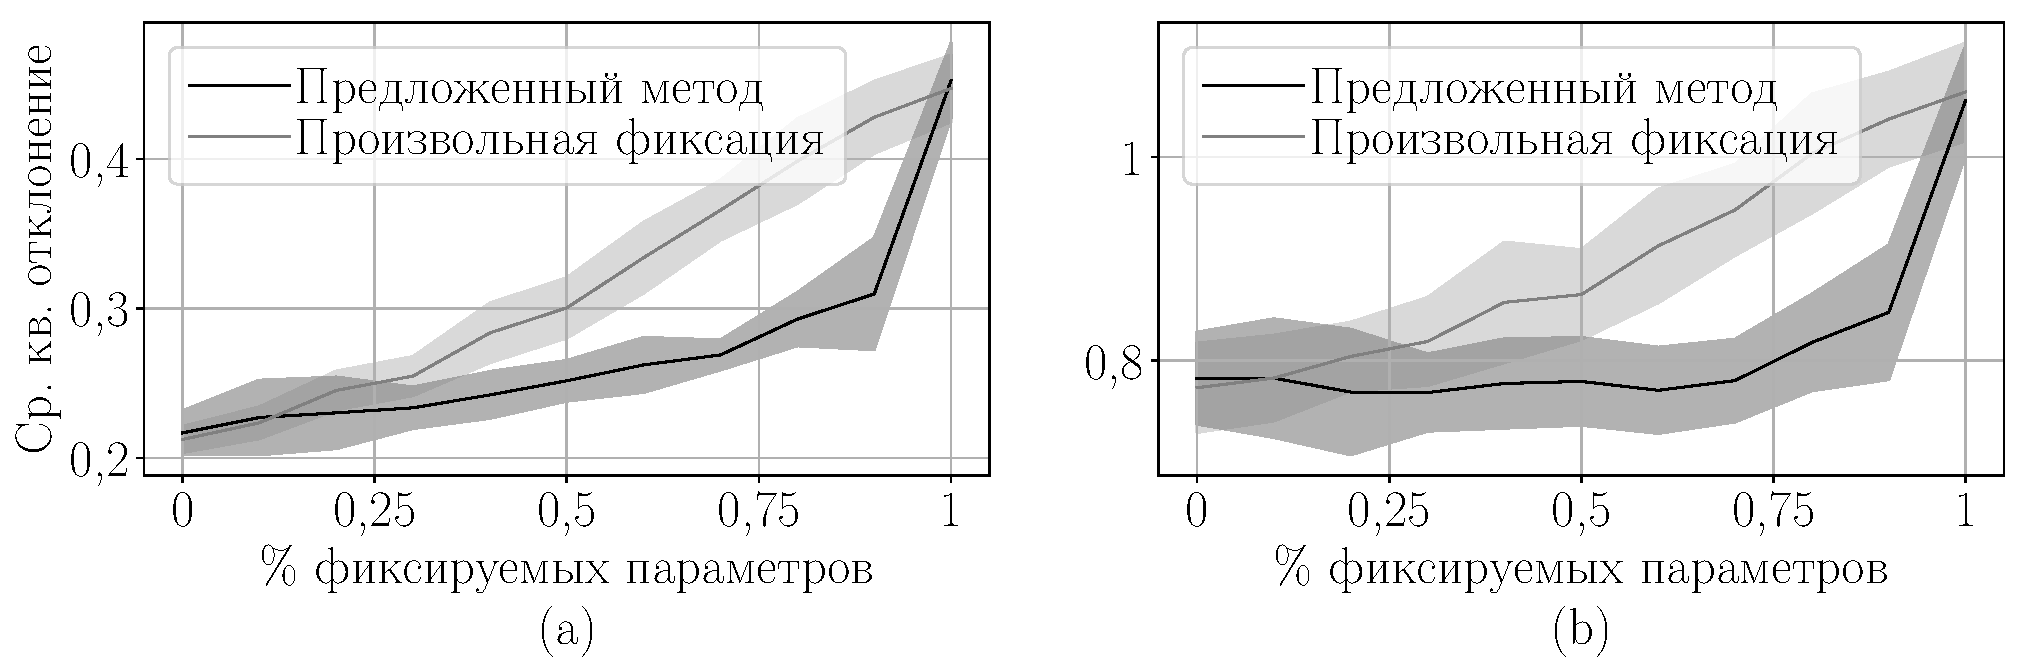
\includegraphics[width=1\textwidth]{results/order/generate_data_neural_loss}
\caption{Зависимость качества модели от числа зафиксированных параметров: a) на обучающей выборке; b) на тестовой выборке}
\label{fg:ex:syn3:1}
\end{figure}

\begin{figure}[h!t]\center
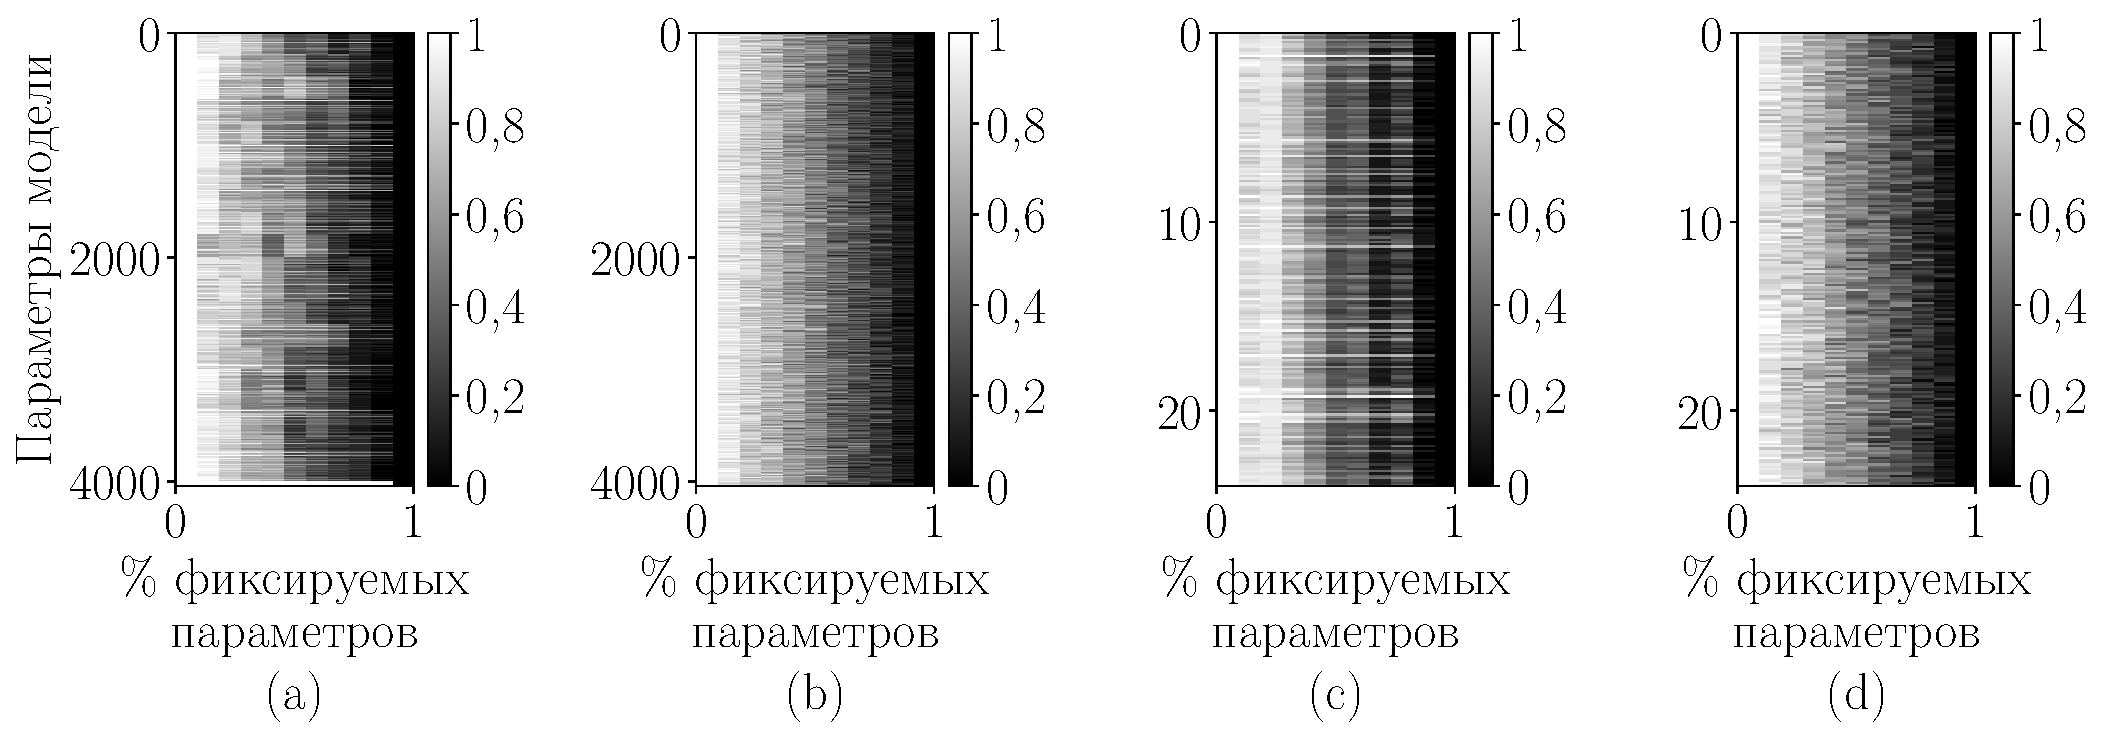
\includegraphics[width=1\textwidth]{results/order/generate_data_neural_matshow}
\caption{Визуализация векторов $\hat{\bm{\alpha}}\bigr(k\bigr)$ в зависимости от числа фиксируемых параметров: a) все параметры модели упорядочены предложенным методом; b) все параметры модели упорядочены произвольным образом; c) часть параметров модели упорядочена предложенным методом; d) часть параметров модели упорядочена произвольным образом}
\label{fg:ex:syn3:2}
\end{figure}

Эксперимент проводился на синтетически построенных данных. В качестве модели использовалась двухслойная нейросеть --- перцептрон.
%На рис. \ref{fg:ex:syn3:1} показано, что фиксация параметров в соответствии с предложенным порядком является лучше, чем фиксация параметров произвольным образом, так как функция ошибки растет медленней при фиксации большего процента параметров.
На рис. \ref{fg:ex:syn3:1} показаны графики зависимости функции потерь $\mathcal{L}$ от числа фиксируемых параметров. В случае фиксации параметров предложенным методом функция потерь $\mathcal{L}$ растет медленней, чем в случае фиксации параметров произвольным образом.

На рис. \ref{fg:ex:syn3:2} показана зависимость векторов $\hat{\bm{\alpha}}\bigr(k\bigr)$ от числа фиксируемых параметров. Каждый столбец соответствует одному вектору $\hat{\bm{\alpha}}\bigr(k\bigr)$. На рис. \ref{fg:ex:syn3:2}a, \ref{fg:ex:syn3:2}с видно, что $\hat{\bm{\alpha}}\bigr(k\bigr)$ имеет большое число компонент вектора, близких к $1$. Так как $\hat{\bm{\alpha}}\bigr(k\bigr)$ является усреднением вектора с компонентами $0$ или $1$, то предложенный порядок задает некоторый устойчивый порядок на множестве параметров модели. На рис. \ref{fg:ex:syn3:2}b, \ref{fg:ex:syn3:2}d видно, что в случае произвольной фиксации параметров компоненты вектора $\hat{\bm{\alpha}}\bigr(k\bigr)$ имеют одинаковые значения, следовательно, никакого порядка на множестве параметров нет.

\paragraph{Выборка Boston Housing.}
\begin{figure}[h!t]\center
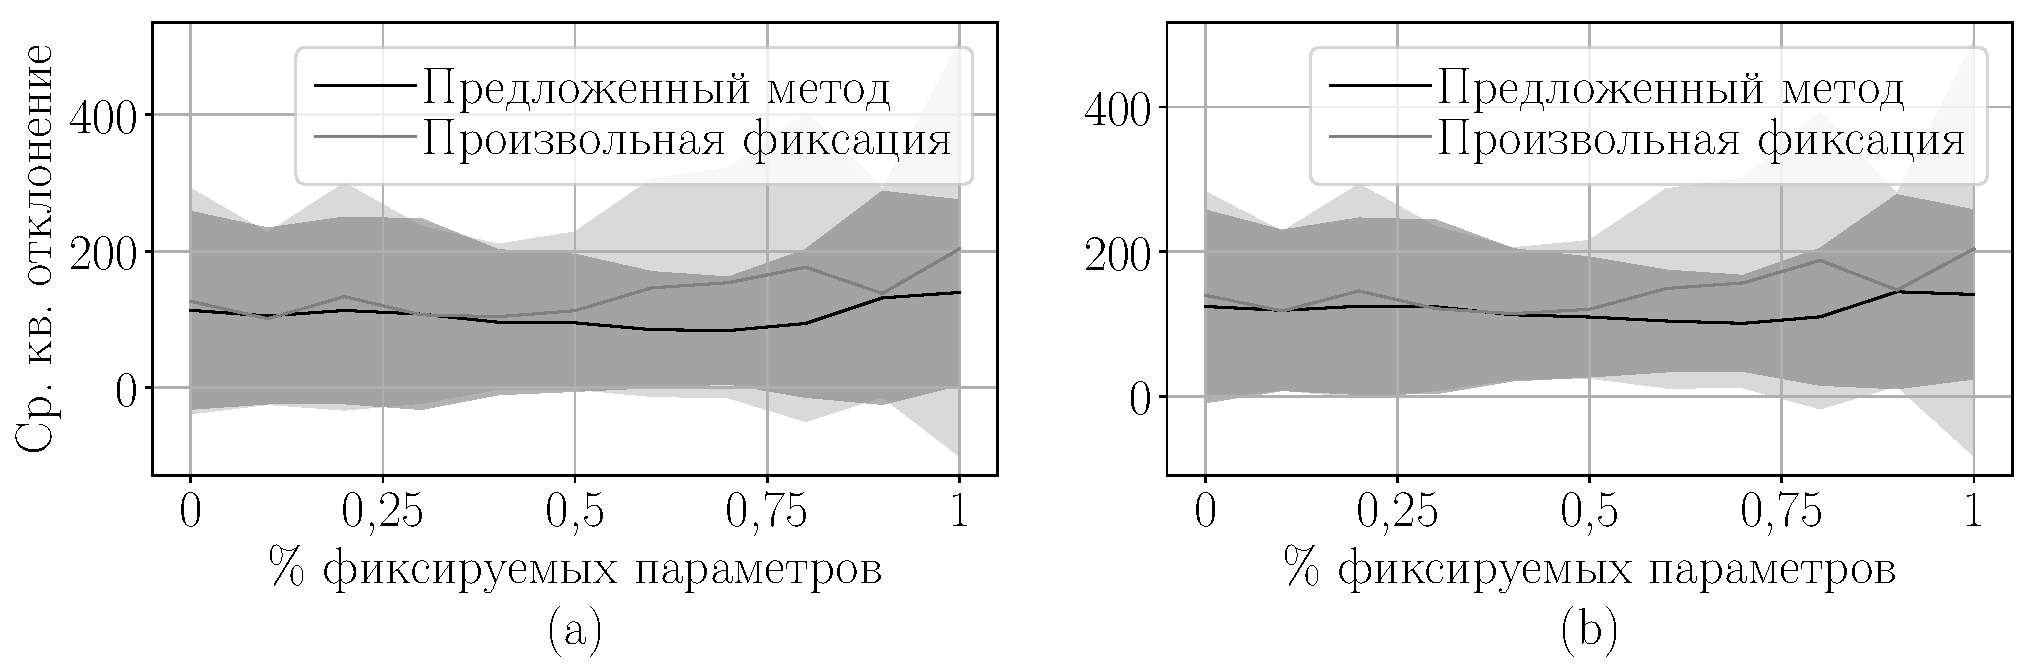
\includegraphics[width=1\textwidth]{results/order/boston_data_loss}
\caption{Зависимость качества модели от числа зафиксированных параметров: a) на обучающей выборке; b) на тестовой выборке}
\label{fg:ex:bost:1}
\end{figure}
Эксперимент проводился на реальных данных.
%На рис. \ref{fg:ex:bost:1} показано, что фиксация параметров в соответствии с предложенным порядком является лучше, чем заморозка параметров произвольным образом, так как функция ошибки растет медленней при фиксации параметров. Также видно, что в случае произвольной фиксации параметров функция ошибки имеет большую дисперсию, что указывает на сильную не устойчивость. Фиксация параметров предложенным методом является более устойчивым, что следует из того, что функция ошибки имеет меньше дисперсию.
На рис. \ref{fg:ex:bost:1} показаны графики зависимости функции потерь $\mathcal{L}$ от числа фиксируемых параметров. В случае фиксации параметров предложенным методом, функция потерь $\mathcal{L}$ растет так же, как и в случае фиксации параметров произвольным образом.
Данный результат следует из того, что нейросеть оказалась избыточно сложной моделью с большим числом параметров. После фиксации значимого числа параметров у модели оставалась большое число параметров для дообучения.

На рис. \ref{fg:ex:bost:2} показана зависимость векторов $\hat{\bm{\alpha}}\bigr(k\bigr)$ от числа фиксируемых параметров. На рис. \ref{fg:ex:bost:2}a, \ref{fg:ex:bost:2}с видно, что $\hat{\bm{\alpha}}\bigr(k\bigr)$ меняется незначительно от запуска к запуску алгоритма. Следовательно, предложенный порядок задает устойчивый к разным запускам порядок на множестве параметров модели. На рис. \ref{fg:ex:bost:2}b, \ref{fg:ex:bost:2}d видно, что в случае произвольной фиксации параметров вектор $\hat{\bm{\alpha}}\bigr(k\bigr)$ является произвольным и никакого порядка на множестве параметров нет.

\begin{figure}[h!t]\center
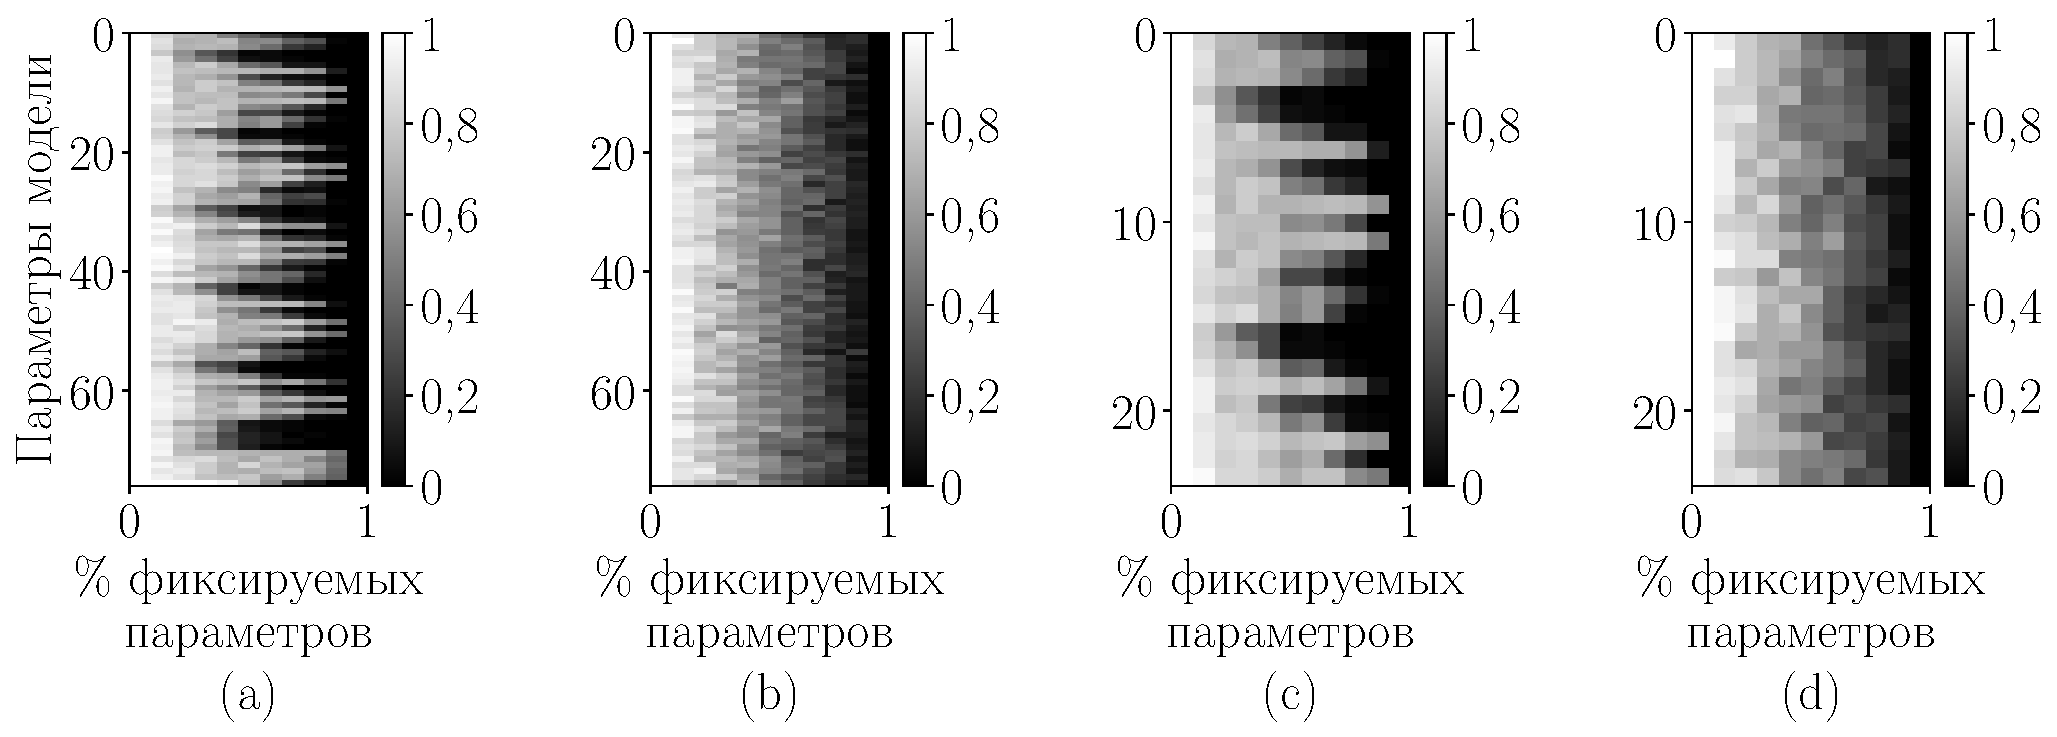
\includegraphics[width=1\textwidth]{results/order/boston_data_matshow}
\caption{Визуализация векторов $\hat{\bm{\alpha}}\bigr(k\bigr)$ в зависимости от числа фиксируемых параметров: a) все параметры модели упорядочены предложенным методом; b) все параметры модели упорядочены произвольным образом; c) часть параметров модели, упорядочена предложенным методом; d) часть параметров модели упорядочена произвольным образом}
\label{fg:ex:bost:2}
\end{figure}

\paragraph{Выборка Synthetic 3.}
\begin{figure}[h!t]\center
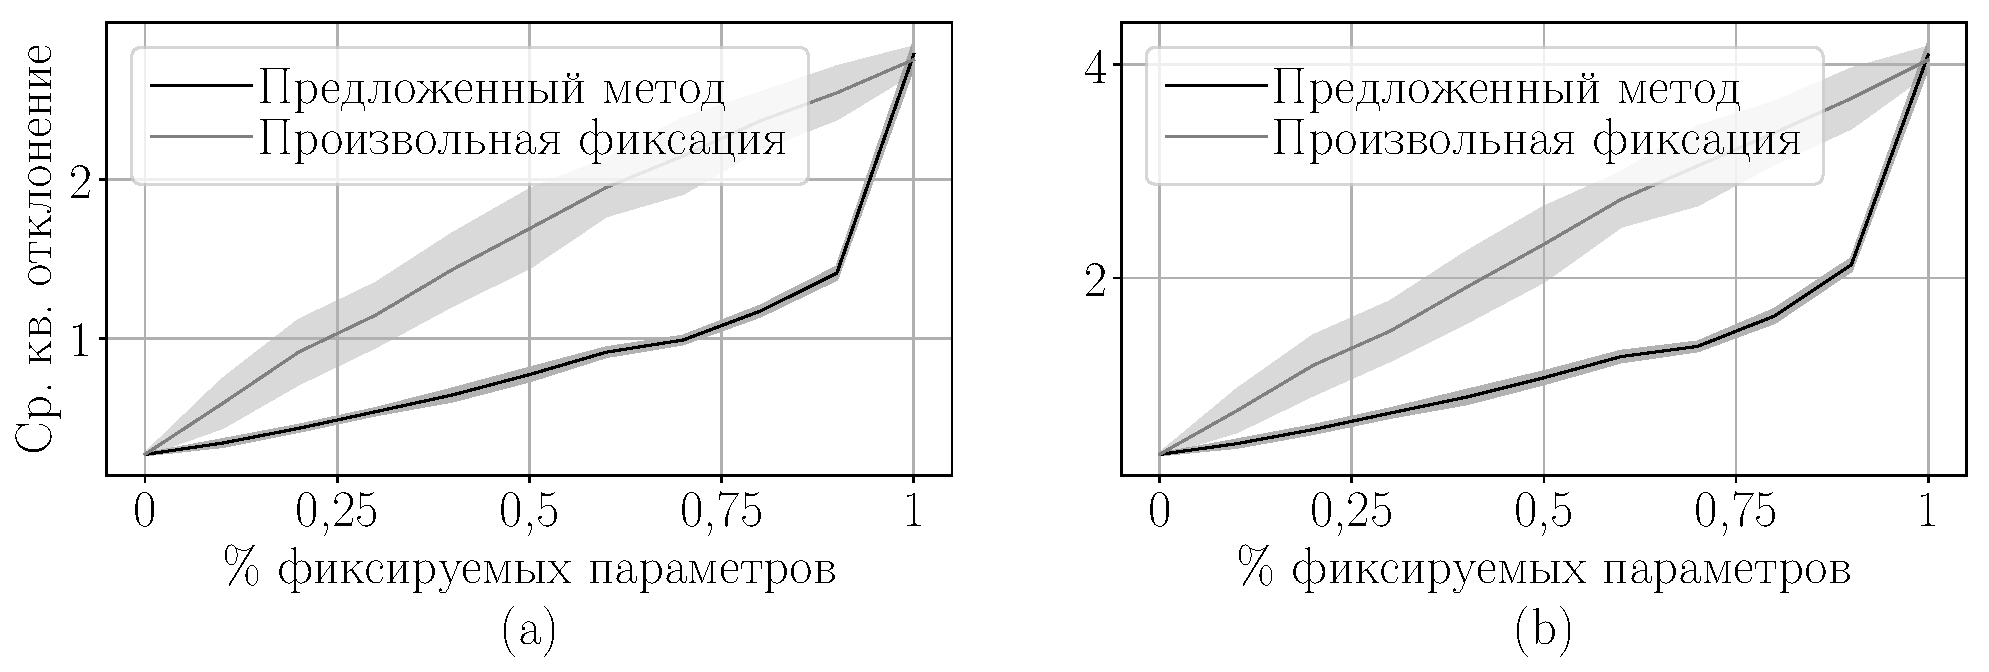
\includegraphics[width=1\textwidth]{results/order/generate_data_linear_loss}
\caption{Зависимость качества модели от числа зафиксированных параметров: a) на обучающей выборке; b) на тестовой выборке}
\label{fg:ex:syn1:1}
\end{figure}

\begin{figure}[h!t]\center
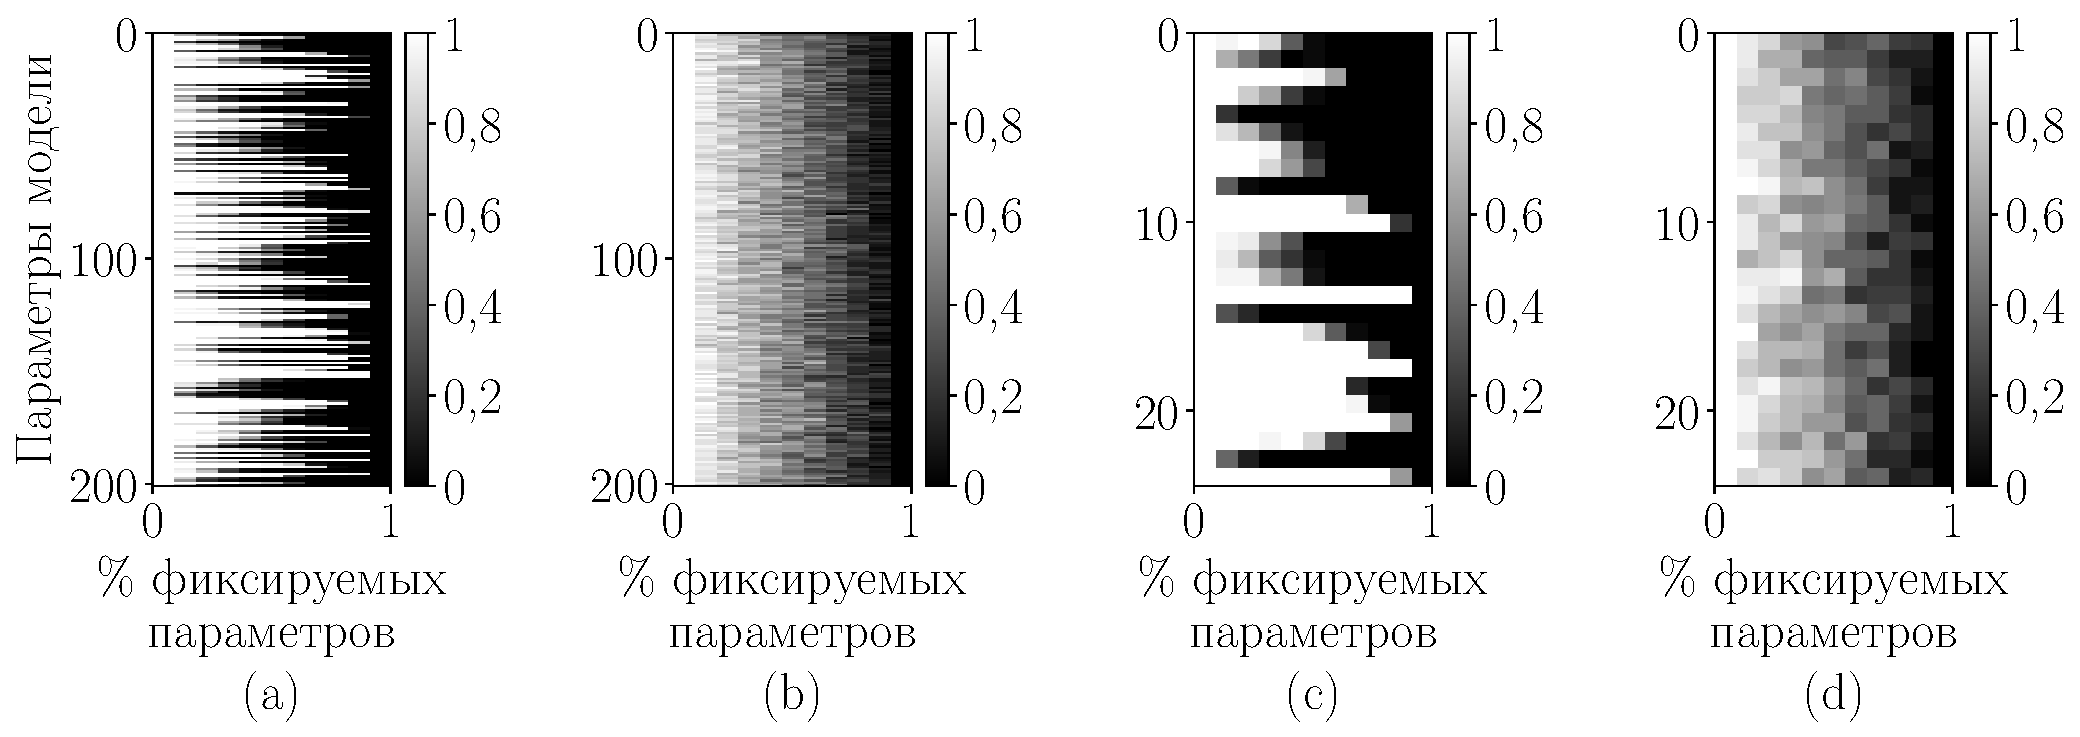
\includegraphics[width=1\textwidth]{results/order/generate_data_linear_matshow}
\caption{Визуализация векторов $\hat{\bm{\alpha}}\bigr(k\bigr)$ в зависимости от числа фиксируемых параметров: a) все параметры модели упорядочены предложенным методом; b) все параметры модели упорядочена произвольным образом; c) часть параметров модели, упорядочены предложенным методом; d) часть параметров модели упорядочена произвольным образом}
\label{fg:ex:syn1:2}
\end{figure}

Эксперимент проводился на синтетически построенных данных. В качестве модели использовалась линейная модель регрессии.
%На рис. \ref{fg:ex:syn1:1} показано, что фиксация параметров в соответсвии с предложенным порядком является лучше, чем фиксация параметров произвольным образом, так как функция ошибки растет медленней при фиксации параметров. Фиксация параметров предложенным методом является более устойчивым, что следует из того, что дисперсия функции ошибки почти отсутствует в отличии от дисперсии функции ошибки, где фиксация параметров производилась произвольным образом.
На рис. \ref{fg:ex:syn1:1} показаны графики зависимости функции потерь $\mathcal{L}$ от числа фиксируемых параметров. В случае фиксации параметров предложенным методом функция потерь $\mathcal{L}$ растет значительно медленней в сравнении со случаем фиксации параметров произвольным образом. Дисперсия функции ошибки также значительно меньше в случае фиксации параметров предложенным методом.

На рис. \ref{fg:ex:syn1:2} показано, что вектора $\hat{\bm{\alpha}}\bigr(k\bigr)$ не меняется от запуска к запуску. Так как данная модель линейная, то порядок на параметрах модели индуцирует некоторый порядок на множестве признаков.

\paragraph{Выборка MNIST.}

\begin{figure}[h!t]\center
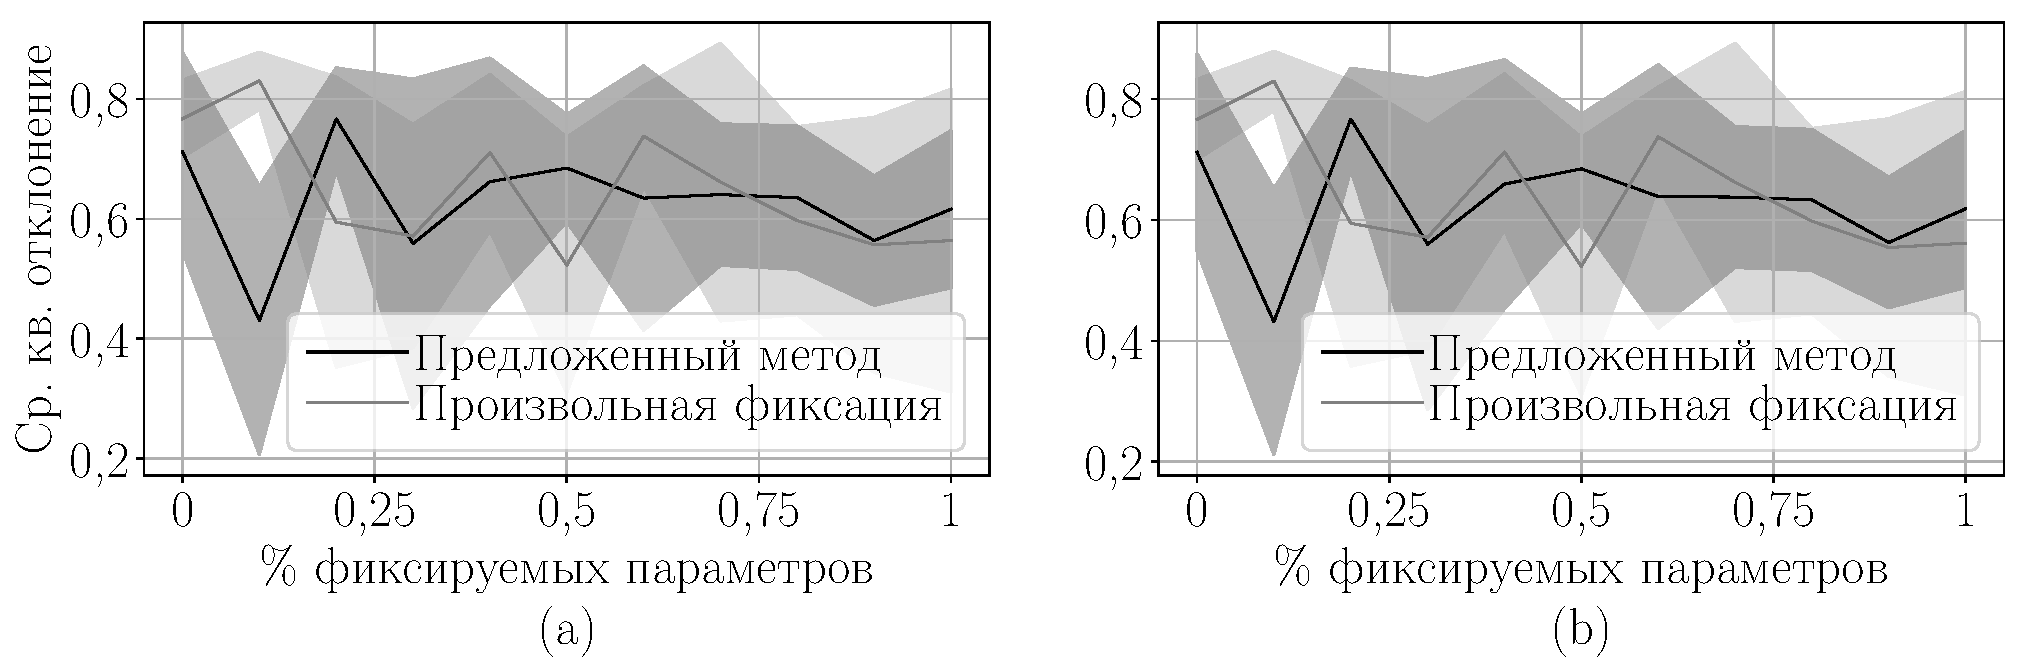
\includegraphics[width=1\textwidth]{results/order/mnist_data_loss}
\caption{Зависимость качества модели от числа зафиксированных параметров: a) на обучающей выборке; b) на тестовой выборке}
\label{fg:ex:mnist:1}
\end{figure}

\begin{figure}[h!t]\center
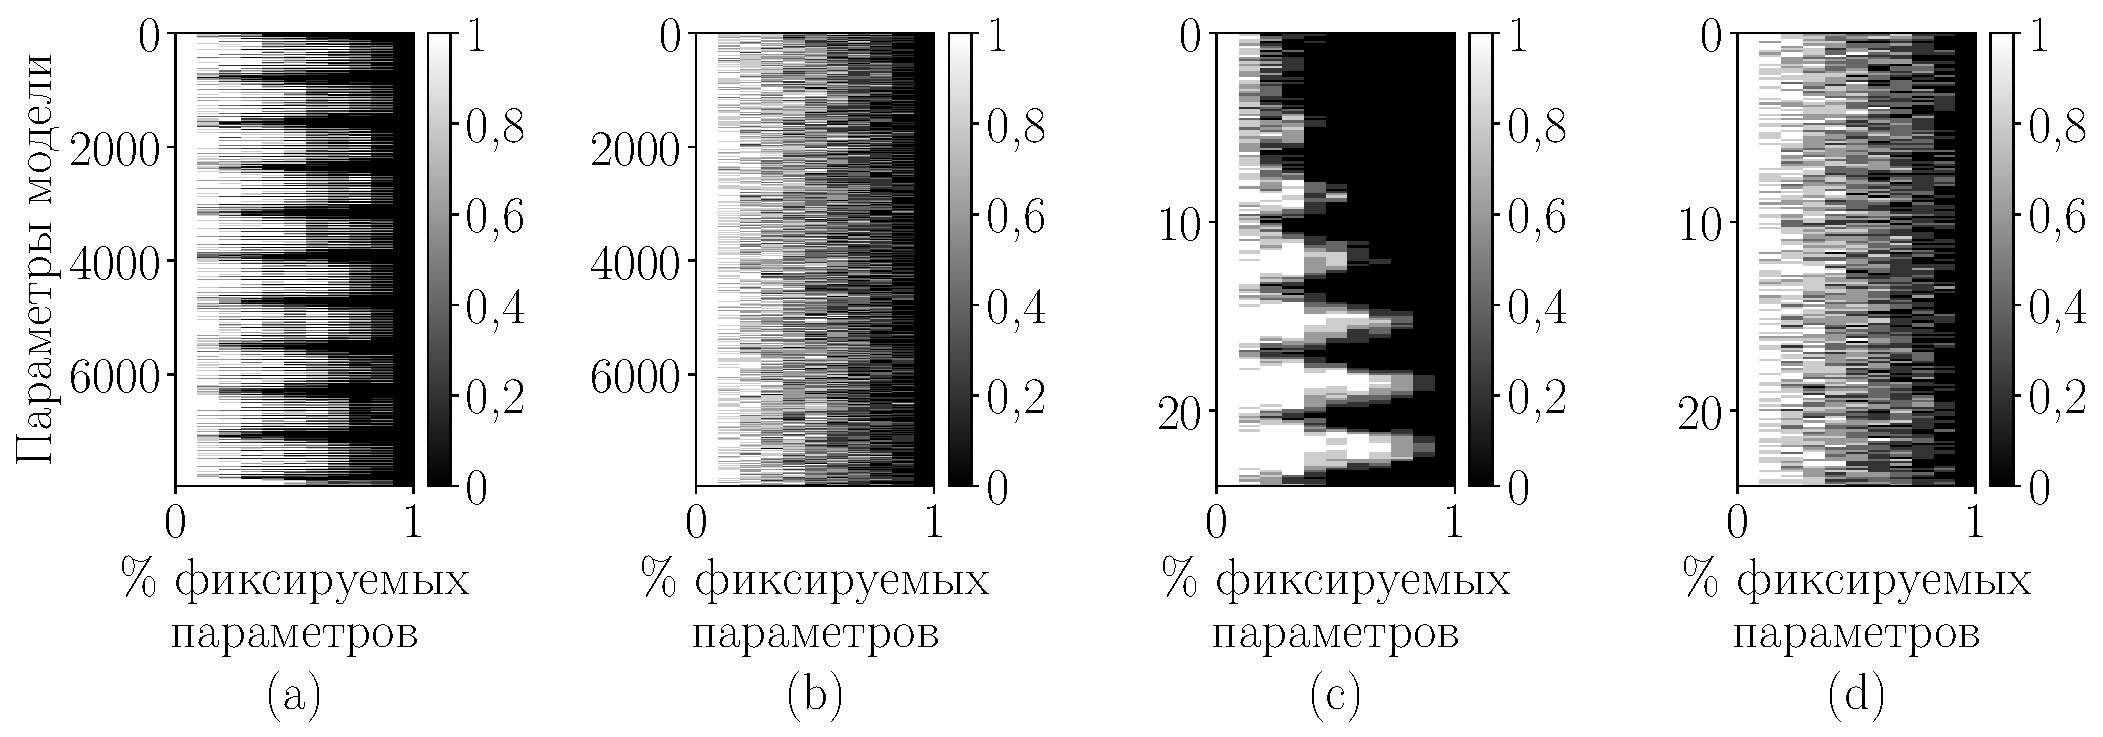
\includegraphics[width=1\textwidth]{results/order/mnist_data_matshow}
\caption{Визуализация векторов $\hat{\bm{\alpha}}\bigr(k\bigr)$ в зависимости от числа фиксируемых параметров: a) все параметры модели упорядочены предложенным методом; b) все параметры модели упорядочены произвольным образом; c) часть параметров модели упорядочена предложенным методом; d) часть параметров модели упорядочена произвольным образом}
\label{fg:ex:mnist:2}
\end{figure}

В эксперименте рассматривался двухслойный перцептрон для классификации изображений. В качестве входных данных рассматривались изображения размера $28\times28$, на которых изображены цифры. 

На рис. \ref{fg:ex:mnist:1} показано, что графики функции ошибки похожи в случае фиксации параметров параметров предложенным методом и в случае произвольной фиксации. Данный результат есть следствие того факта, что нейросеть является заведомо переусложненной моделью с большим числом параметров. После фиксации большого числа параметров у нейросети все еще остается значимое число параметров модели для дообучения.

На рис. \ref{fg:ex:mnist:2} показано, что в случае модели со значимым числом оптимизационных параметров,предложенный метод упорядочения параметров устойчив от запуску к запуску.

